\section*{Exercise 4}
\subsection*{a)}\small The Certer is underlined.\normalsize

\paragraph{Round 1}~\newline
Cluster 1: $\underline{A}$\\
Cluster 2: $\underline{B}$\\
Cluster 3: $\underline{C},D,E,F,G,H$

\paragraph{Round 2}~\newline
Cluster 1: $\underline{A}$\\
Cluster 2: $\underline{B},C$\\
Cluster 3: $\underline{(7.5,6)},D,E,F,G,H$

\paragraph{Round 3}~\newline
Cluster 1: $\underline{A},B$\\
Cluster 2: $\underline{(3,9.5)},C$\\
Cluster 3: $\underline{(8.5,5.6)},D,E,F,G,H$

\paragraph{Round 4}~\newline
Cluster 1: $\underline{(3.5,11.5)},A,B$\\
Cluster 2: $\underline{C}$\\
Cluster 3: $\underline{(8.5,5.6)},D,E,F,G,H$\\
The clustering of the Points stays the same as the roud before so the algorithm halts.

\subsection*{b)}
\begin{center}
  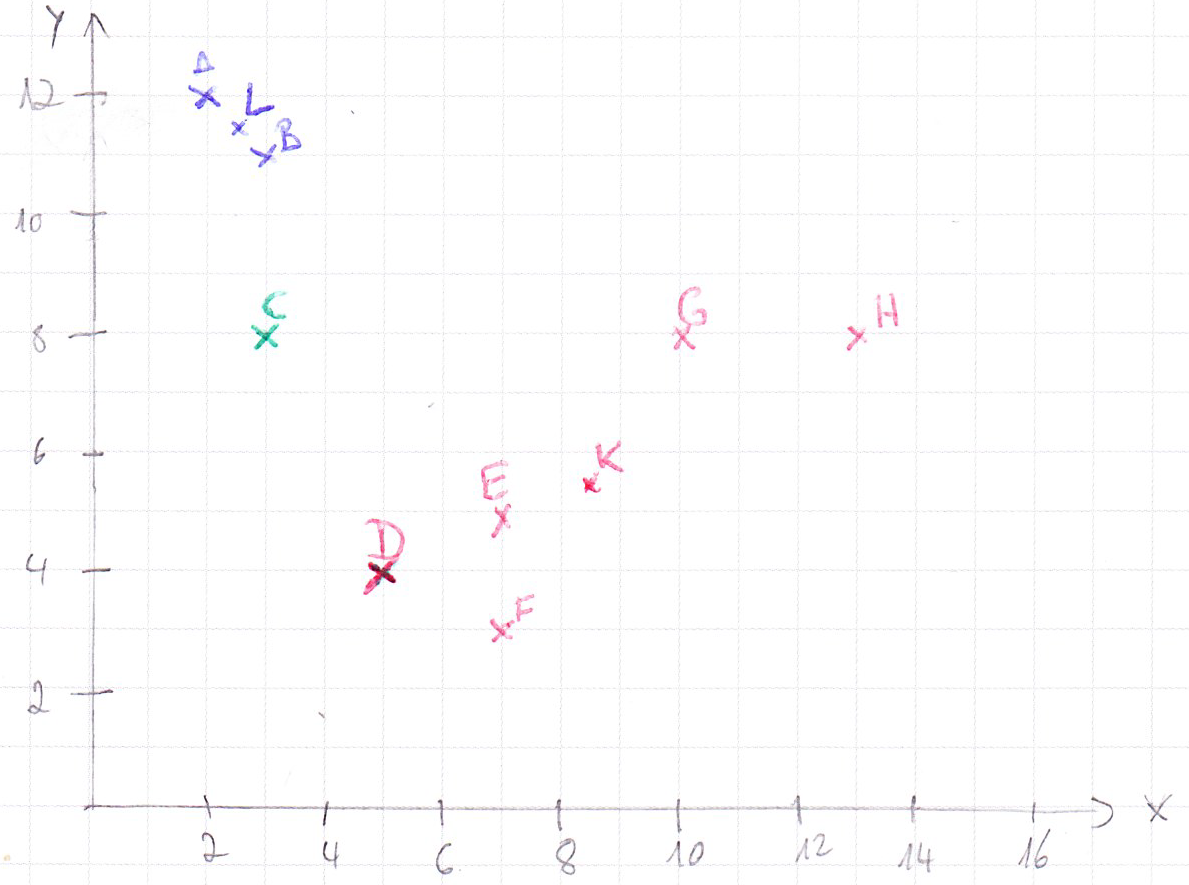
\includegraphics[width=0.7\linewidth]{E4_diag}\\
  \small $L$ is mean of cluster 1: $(2.5,11.5)$, $C$ is mean of cluster 2: $(3,8)$, K is mean of cluster 3: $(8.5,5.6)$
\end{center}
